\null\newpage
\clearpage

\section{Anexo}

\subsection{Diseños preliminares - imágenes}

\begin{figure}[htb]
    \centering
    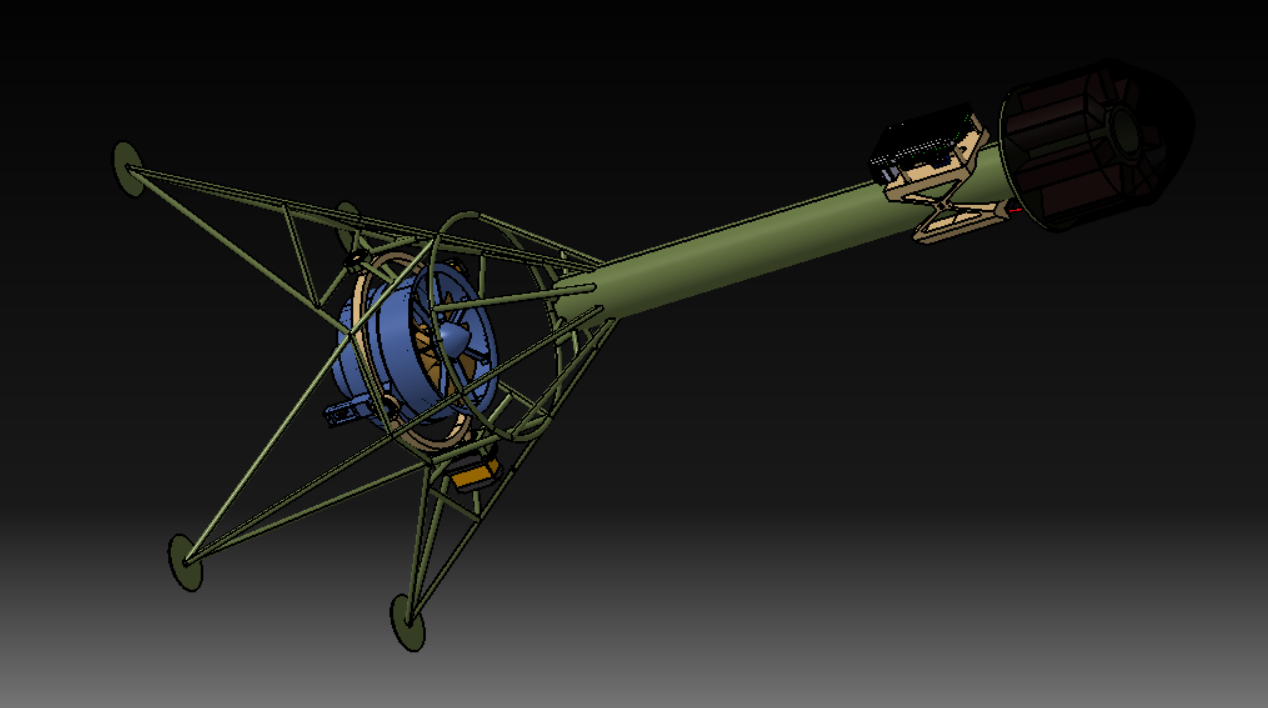
\includegraphics[height=0.25\pdfpageheight]{fig/design/0}
    \caption{Prototipo de fuselaje con patas reticuladas integro en aluminio, baterías en la nariz, aviónica debajo de la nariz, sin sistema anti rolido.}
    \label{fig:design/0}
\end{figure}


\begin{figure}[htb]
    \centering
    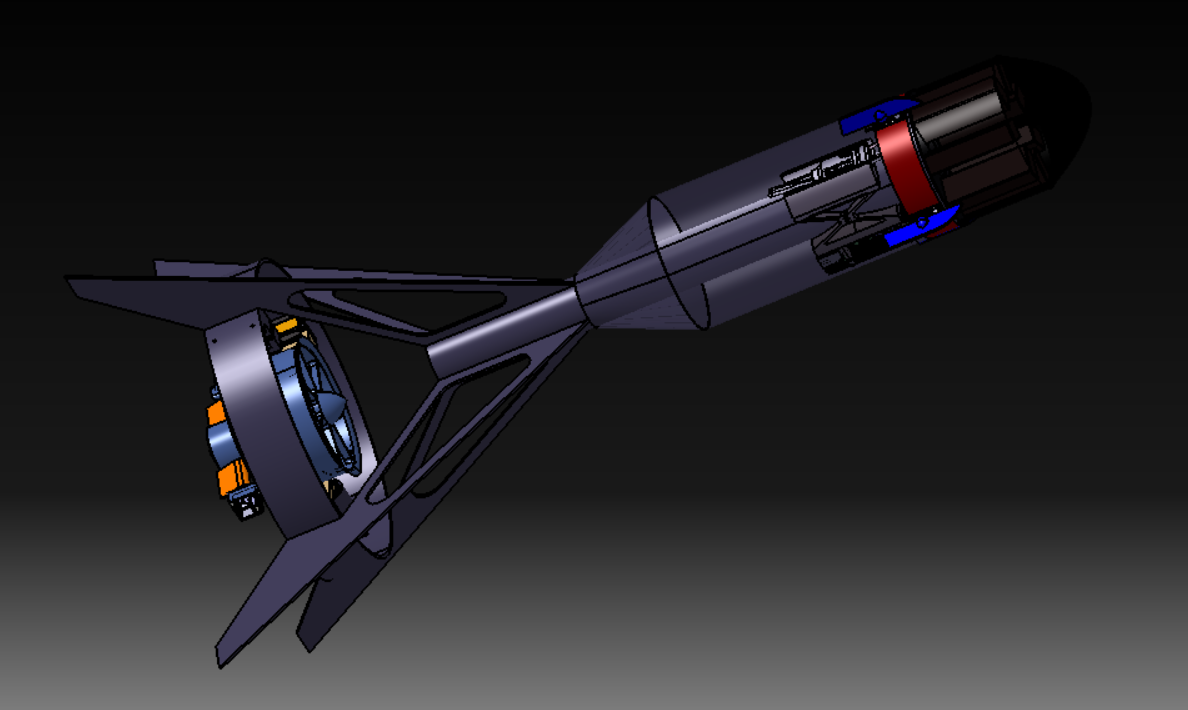
\includegraphics[width=\linewidth]{fig/design/1}
    \caption{Prototipo evolución al fuselaje de aluminio tubular, baterías en la nariz, sistema anti rolido en
    la parte superior, aviónica debajo de las baterías.}
    \label{fig:design/1}
\end{figure}

\begin{figure}[htb]
    \centering
    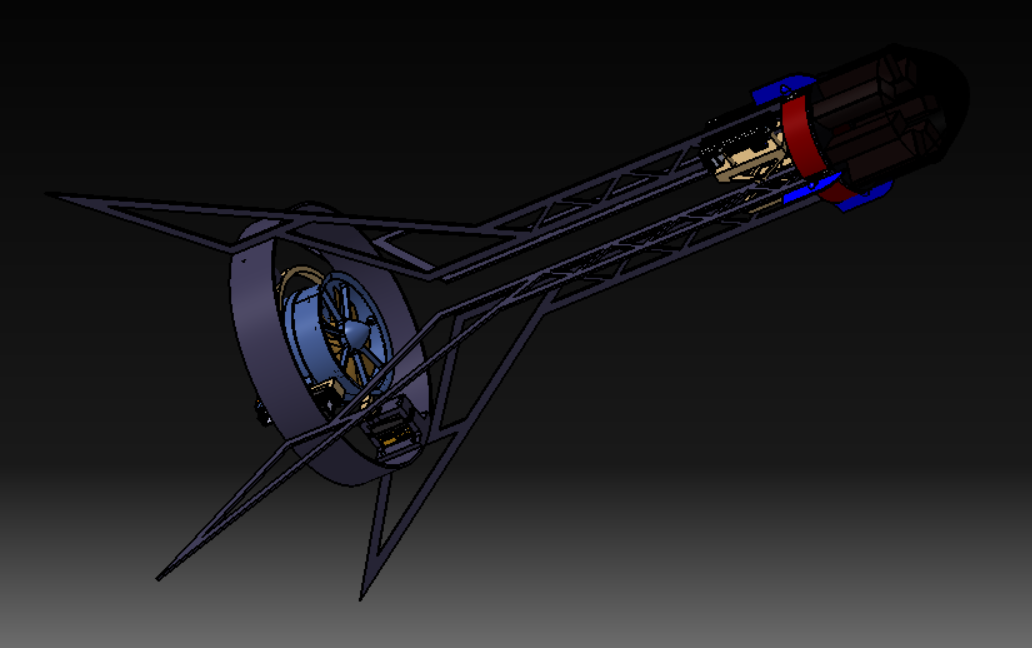
\includegraphics[width=\linewidth]{fig/design/2}
    \caption{Prototipo fuselaje reticulado de aluminio en forma de placas, baterías en la nariz, sistema anti
    rolido en la parte superior, aviónica debajo de las baterías.}
    \label{fig:design/2}
\end{figure}

\begin{figure}[htb]
    \centering
    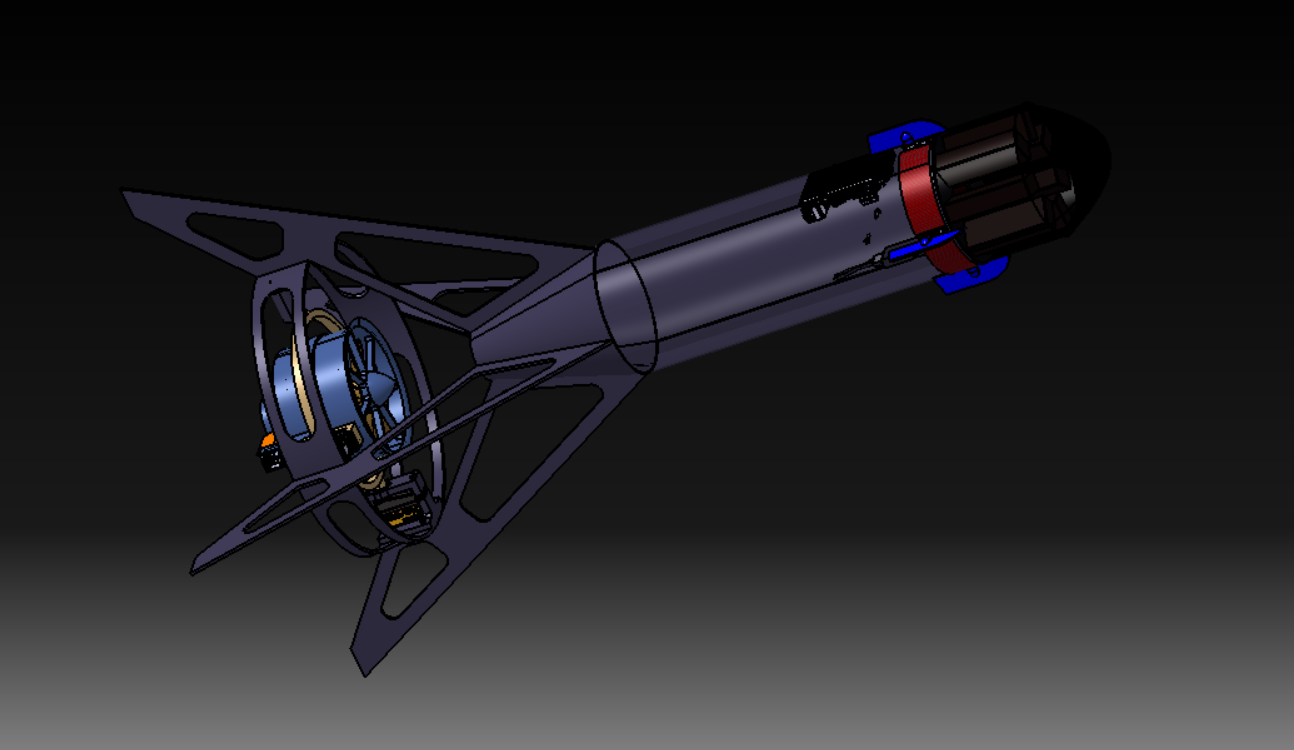
\includegraphics[width=\linewidth]{fig/design/3}
    \caption{Prototipo fuselaje tubular conico, para favorecer la admision del EDF, patas vaciadas, beterias en la nariz, sistema antirolido en la parte superior,  avionica por debajo de las baterias.}
    \label{fig:design/3}
\end{figure}

\begin{figure}[htb]
    \centering
    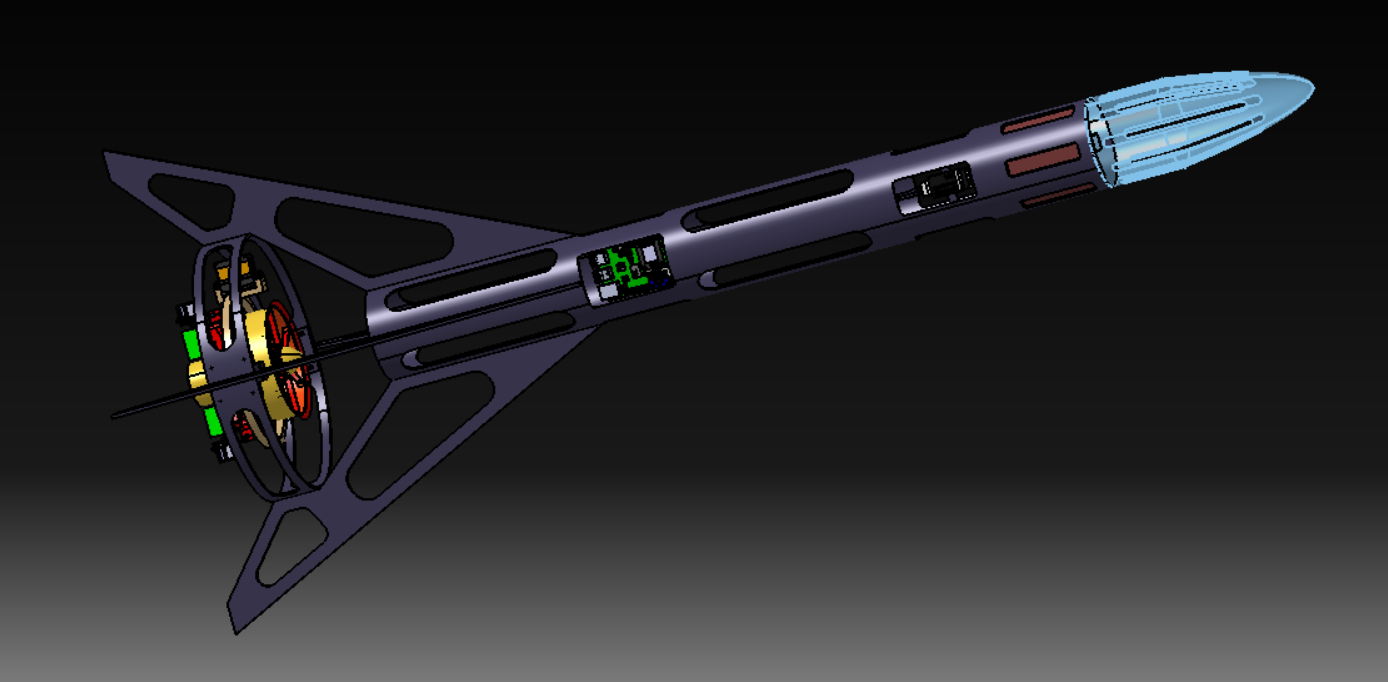
\includegraphics[width=\linewidth]{fig/design/4}
    \caption{Un diseño previo al diseño final. Los vaciados son distintos y la disposición de componentes es distinta. La posición de la Raspberry Pi fue cambiada luego de la charla con Pablo Cosutta. Puntualmente la charla evidencio un posible problema de interferencia electromagnetica al la Raspberry Pi tan cerca de los cables trifásicos de los ESC. Por lo que se decidió mover la Raspberry Pi a la parte superior del fuselaje.}
    \label{fig:design/4}
\end{figure}

\begin{figure}[htb]
    \centering
    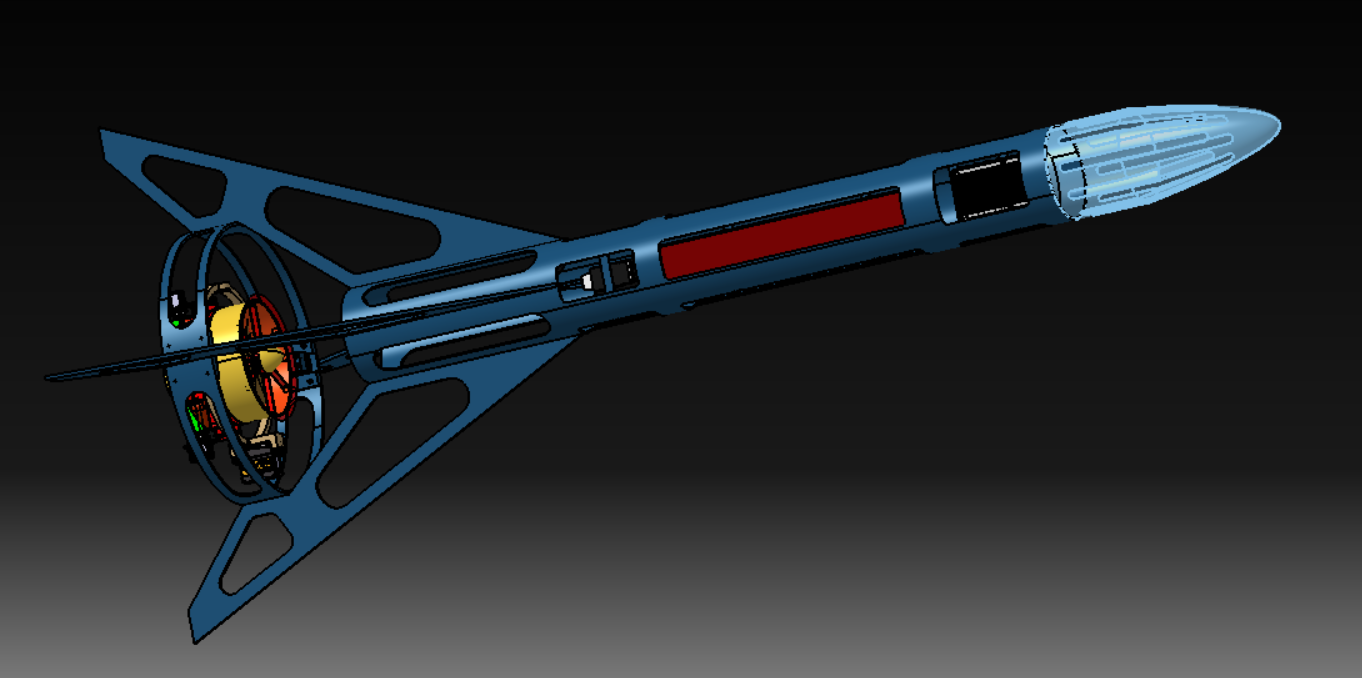
\includegraphics[width=\linewidth]{fig/design/5}
    \caption{Prototipo fuselaje de aluminio tubular vaciado, baterías en el cuerpo, en el núcleo, nariz aerodinámica, patas optimizadas, aviónica en la parte superior, sistema anti-rolido en la parte
    inferior del EDF por derivación del flujo.}
    \label{fig:design/5}
\end{figure}

\null\newpage
\clearpage
